\documentclass[10pt,t]{beamer}

% fonts
\usefonttheme{professionalfonts}
\usepackage[osf, sc]{mathpazo} % for rm
\usepackage{courier} % for mono
% \usepackage[euler-digits]{eulervm}
\usefonttheme{serif}
% more about eulervm:
% \mathrm -> rmdefault
% \mathbf -> bfdefault
% \mathsf -> sfdefault
% \mathtt -> ttdefault
% Thus, you should redefine the default text fonts before loading the eulervm package!
% redefine: \mathit, \mathbold, \mathcal

%math
\usepackage{amsmath}
\DeclareMathOperator*{\argmin}{arg\,min}
\DeclareMathOperator*{\argmax}{arg\,max}
\newcommand*\diff{\mathop{}\!\mathrm{d}}
% color
\definecolor{brown}{rgb}{0.4, 0.208, 0.192}
\definecolor{gray1}{rgb}{0.125, 0.125, 0.125}
\definecolor{gray2}{rgb}{0.157, 0.157, 0.157}
\definecolor{green2}{rgb}{0.16862745098039217,0.4,0.19607843137254902}
\definecolor{blue2}{rgb}{0,0.40784313725490196,0.6352941176470588}
\definecolor{brown2}{rgb}{0.6235294117647059,0.2901960784313726,0}

\definecolor{blue}{rgb}{0.18, 0.2, 0.529}
\definecolor{orange}{RGB}{206,117,59} % used for strong
\definecolor{green}{RGB}{49,104,108} % used for everywhere, link,...
\definecolor{red}{RGB}{133,60,66}
\definecolor{pink}{RGB}{184,86,150}



\setbeamercolor{caption name}{fg=green}

% settings for itemize and enumerate
\setbeamertemplate{itemize item}{\textbullet}
\setbeamertemplate{itemize subitem}{\bfseries --}
\setbeamertemplate{itemize subsubitem}{$\circ$}
\setbeamercolor{itemize item}{fg=green}
\setbeamercolor{itemize subitem}{fg=brown}
\setbeamercolor{itemize subsubitem}{fg=gray2}

\setbeamertemplate{enumerate item}{\arabic{enumi}.}
\setbeamertemplate{enumerate subitem}{(\roman{enumii})}
\setbeamertemplate{enumerate subsubitem}{\alph{enumiii}.}
\setbeamercolor{enumerate item}{fg=green}
\setbeamercolor{enumerate subitem}{fg=brown}
\setbeamercolor{enumerate subsubitem}{fg=gray2}
% main page style
\setbeamercolor{background canvas}{bg=white}
\setbeamercolor{normal text}{fg=black}
\setbeamertemplate{footline}[frame number]
\setbeamertemplate{navigation symbols}{}
\setbeamercolor{block title}{bg=green!90!black,fg=white}
\setbeamercolor{block body}{bg=green!10}
% frametitle
\setbeamertemplate{frametitle}
{
    \vskip 5pt
    \strut\Large\textcolor{green}{\insertframetitle}\strut
    \ifx\insertframesubtitle\empty
    \vskip-1.7ex
    \textcolor{green}{\hrule height0pt depth0.5pt \relax}
    \else
    \vskip-1ex
    \strut\small\textcolor{green}{\insertframesubtitle}\strut
    \textcolor{green}{\hrule height0pt depth0.5pt \relax}
    \fi
}
% titlepage
\setbeamertemplate{title page}
{
  \makebox[\textwidth][c]{
    \begin{minipage}[b][0.75\paperheight][c]{0.9\textwidth}
      \centering
      \huge\rm\inserttitle\\
      \Large\rm\insertsubtitle
      \vskip-1.5ex
      \textcolor{green}{\hrule height0pt depth0.8pt \relax}
      \vskip5pt
      \rm\normalsize\insertauthor
    \end{minipage}
  }

  \makebox[\textwidth][c]{
    \begin{minipage}[b][0.25\paperheight][c]{0.4\textwidth}
      \centering
      \rm\insertinstitute
      \par
      \rm\insertdate
    \end{minipage}
  }
}

\usepackage{hyperref}

\usepackage{booktabs}
% ********************************************************************
% tikz
% ********************************************************************
\usepackage{tikz}
\usetikzlibrary{positioning}
\usetikzlibrary{decorations.markings}
\usepackage{pgfplots}






\title{Empirical Asset Pricing \\ Problem Set $1$}
\author{Yu Zhou, HKUST}
\date{\today}


\begin{document}

\maketitle

\begin{frame}{Data sources}
\begin{itemize}
  \item Annual value-weighted market return with and without dividends (all markets: nyse, amex and nasdaq)
  \begin{itemize}
    \item Source: WRDS $\rightarrow$ CRSP $\rightarrow$ Index/Stock File Indexes $\rightarrow$ Market Cap.~- Annual $\rightarrow$ vwretd and vwretx
    \item Time range: 1925--2019
  \end{itemize}
  \item Risk-free rate
  \begin{itemize}
    \item Source: \href{http://www.hec.unil.ch/agoyal/docs/PredictorData2019.xlsx}{Amit Goyal's website}
    \item Time range: 1871--2019
  \end{itemize}
  \item cay
  \begin{itemize}
    \item $cay_t = c_t - \omega a_t - (1 - \omega) y_t$ (see \href{https://onlinelibrary.wiley.com/doi/full/10.1111/0022-1082.00347}{Lettau and Ludvigson (2001, JF))}
    \item Source: \href{https://sites.google.com/view/martinlettau/data}{Martin Lettau's website}
    \item Time range: 1952--2019
  \end{itemize}
\end{itemize}
\end{frame}



\begin{frame}{Q1: Assembling data}
\begin{figure}[h!]
\centering
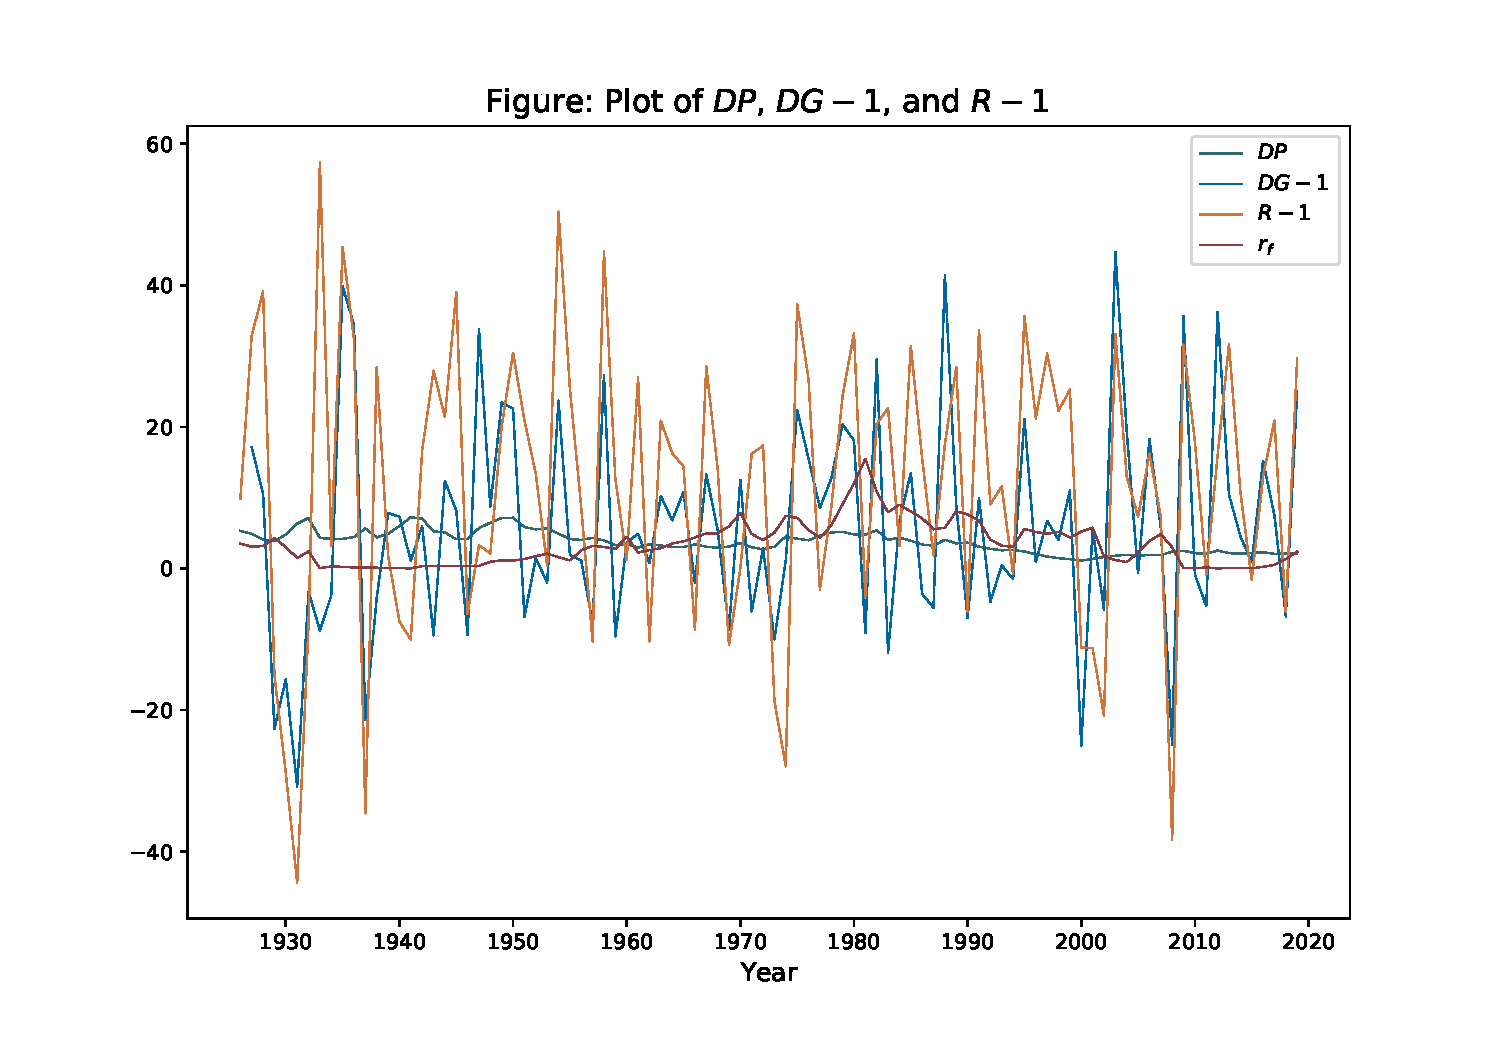
\includegraphics[width=0.8\linewidth]{q1fig1.pdf}
\caption{From the plot, we can see that the dividend growth rates and stock returns are quite volatile. In constrast, the dividend yield and risk-free rates moves slowly.}
\end{figure}
\end{frame}

\begin{frame}{Q1: Assembling data (cont'd)}
\begin{itemize}
  \item mean and standard deviation of returns and dividend growth rate:
\begin{table}
\begin{tabular}{lcc}
\toprule
& $R - 1$ & $DG - 1$ \\
\cmidrule{1-3}
mean & $11.78\%$ & $5.89\%$ \\
std & $0.2$ & $0.15$ \\
\bottomrule
\end{tabular}
\end{table}
\item Sharpe ratio is $0.42$.
\end{itemize}
\end{frame}


\begin{frame}{Q2: Forecasting regressions}
\begin{table}
\footnotesize
\begin{tabular}{lcccccccccc}
\toprule
& 1 & 2 & 3 & 4 & 5 & 6 & 7 & 8 & 9 & 10\\
\cmidrule{1-11}
\multicolumn{11}{l}{Return} \\
$b$ & 2.97 & 5.91 & 8.86 & 12.45 & 14.65 & 18.44 & 23.75 & 29.60 & 36.00 & 44.33 \\
$R^2$ & 0.05 & 0.09 & 0.13 & 0.15 & 0.15 & 0.19 & 0.23 & 0.25 & 0.27 & 0.29 \\
\multicolumn{11}{l}{Excess return} \\
$b$ & 3.11 & 6.17 & 9.23& 12.93 & 15.29 & 19.28 & 24.84 & 31.03 & 37.96 & 46.86 \\
$R^2$ & 0.05 & 0.09 & 0.13 & 0.15 & 0.16 & 0.20 & 0.25 & 0.28 & 0.31 & 0.34 \\
\multicolumn{11}{l}{Dividend growth} \\
$b$ & -0.27 & -0.96 & -1.41 & -1.63 & -2.04 & -2.62 & -2.69 & -2.41 & -2.84 & -3.12\\
$R^2$ & 0 & 0 & 0.01 & 0.01 & 0.01 & 0.01 & 0.01 & 0.01& 0.01 & 0.01\\
\bottomrule
\end{tabular}
\caption{Both coefficients and $R^2$ of returns on dividend yield increases with horizons. This fact implies that dividend yield can predict one-period returns. And one-period return predictability persists. In constrast, the dividend growth rate can not be predicted using dividend yield.}
\end{table}
\end{frame}

\begin{frame}{Q2: Forecasting regressions (cont'd)}
\begin{itemize}
  \item The OLS coefficients and $R^2$ are not biased. But the standard errors and t-statistics are biased because there is autocorrelation between resisual terms for overlapping data.
\end{itemize}
\end{frame}


\begin{frame}{Q2: Hansen-Hodrick Errors}
\begin{itemize}
  \item When run forecasting regressions of overlapping long-horizon returns on variables, heteroskedasticity and autocorrelation in residual terms arise:
  \begin{itemize}
    \item $R_{t\rightarrow t+k} =\Pi_{i = 1}^{k} R_{t+i}$, $R_{t + 1\rightarrow t+1+k} =\Pi_{i = 1}^{k} R_{t+1+i}$, $Cov(R_{t\rightarrow t+k}, R_{t + 1\rightarrow t+1+k}) \neq 0$.
    \item It's natrual to consider the covariance of residual terms as following form:
    $$
    S = \frac{1}{n}E\bigg(\sum_{i,j} x_i x_j^T \varepsilon_i \varepsilon_j\bigg)
    = \frac{1}{n}E\bigg(\sum_{\vert i-j\vert < k} x_i x_j^T \varepsilon_i \varepsilon_j\bigg)
    $$
  \end{itemize}
  \item I Realized it using Python.
\end{itemize}
\end{frame}


\begin{frame}{Q2: Forecasting regressions (cont'd)}
\begin{table}
\begin{tabular}{lcccccccccc}
\toprule
& 1 & 2 & 3 & 4 & 5 & 6 & 7 & 8 & 9 & 10\\
\cmidrule{1-11}
$t_{OLS}$ & 2.32 & 3.45 & 3.66 & 3.85 & 4.52 & 5.08 & 5.88 & 6.73 & 6.94 & 6.97 \\
$t_{HH}$ & 2.32 & 2.70 & 2.92& 3.06 & 3.09 & 2.71& 2.93 & 3.15 & 3.08& 3.25 \\
$t_{NO}$ & 2.32 & 2.27 & 2.39 & 2.16 & 2.02 & 2.35 & 2 & 3.53& 2.54 & 1.66\\
\bottomrule
\end{tabular}
\caption{The standard errors for Hansen-Hodrick estimator and non-overlapping estimator are smaller than the OLS estimator. The one-period return predictability is less strong and persistent than before.}
\end{table}
\end{frame}

\begin{frame}{Q2: Forecasting regressions (cont'd)}
\begin{figure}[h!]
\centering
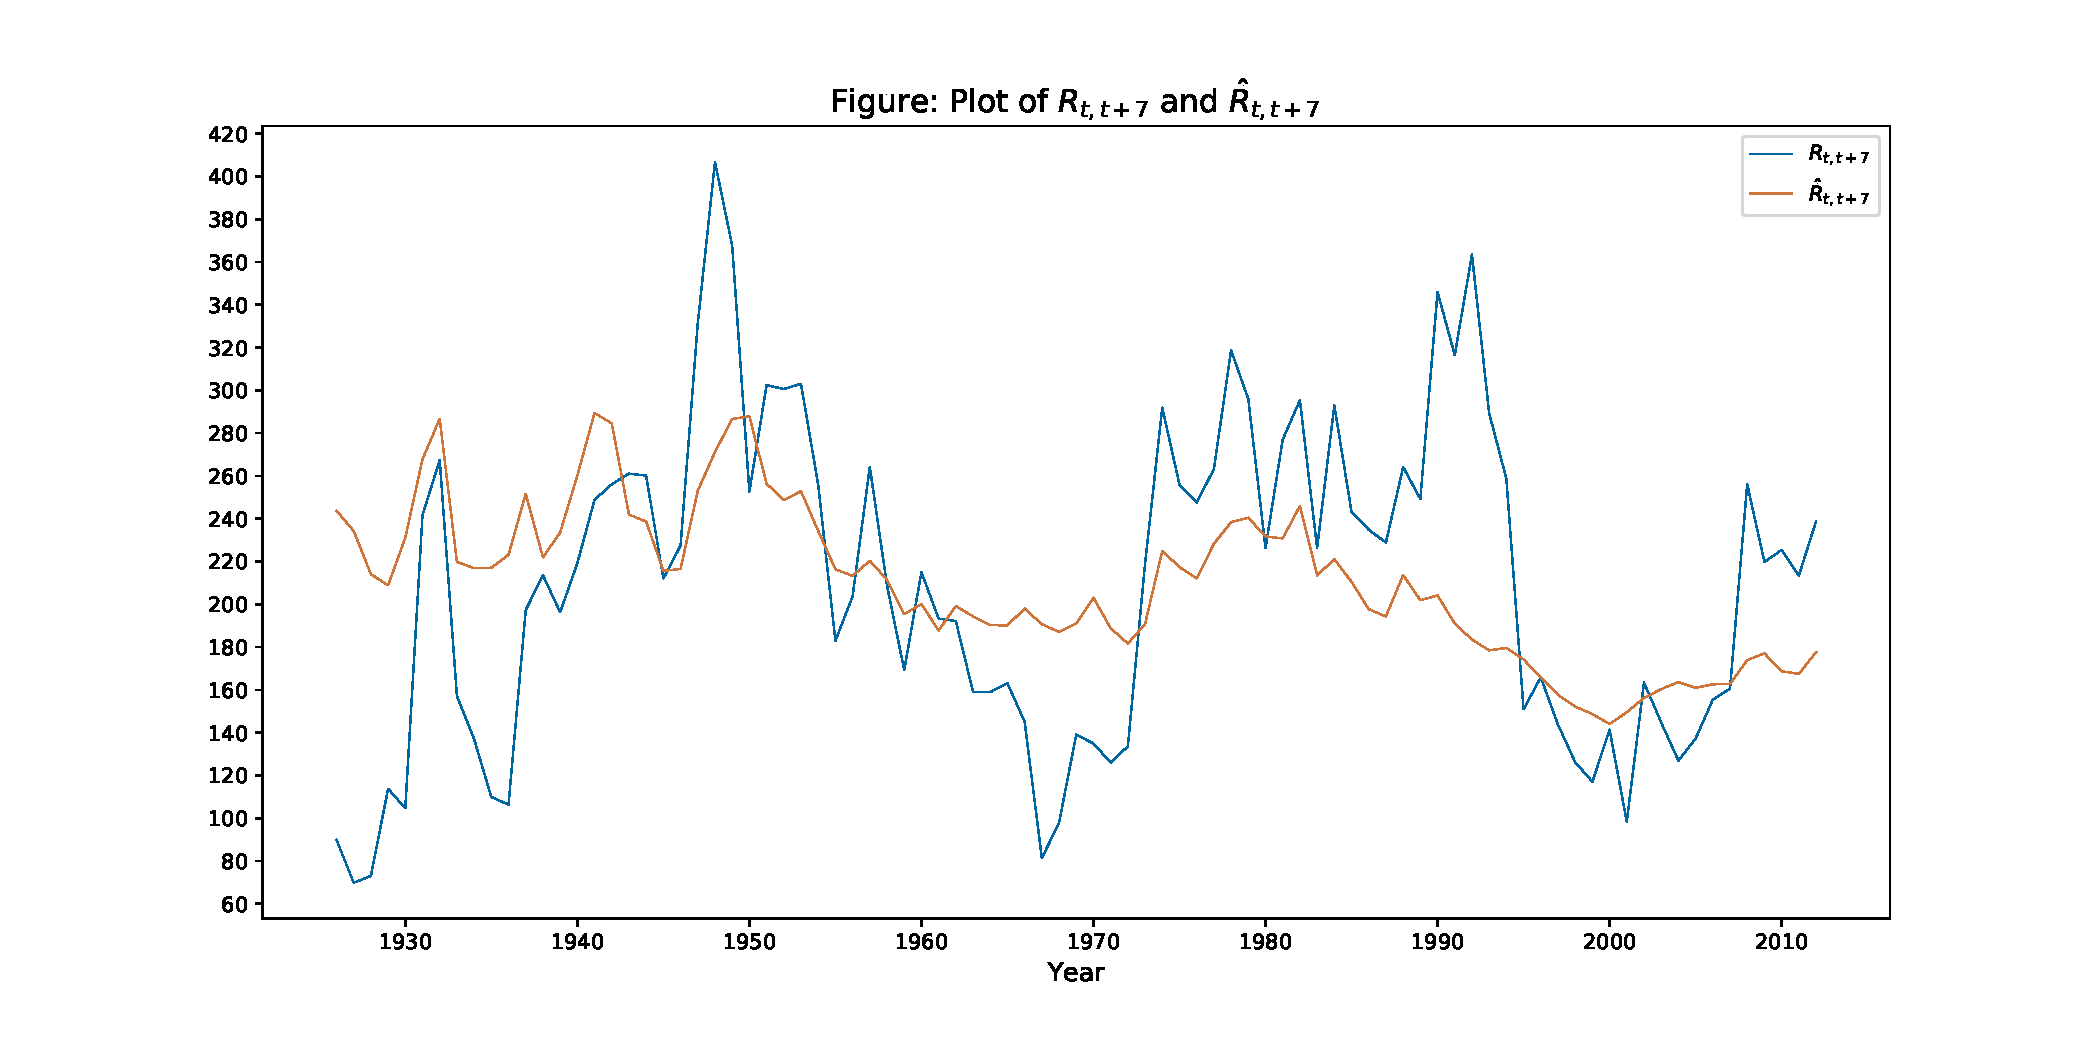
\includegraphics[width=\linewidth]{q2fig1.pdf}
\caption{This figure shows realized and predicted returns. It suggests that return seems to be predictable.}
\end{figure}
\end{frame}

\begin{frame}{Q2: Forecasting regressions (cont'd)}
\begin{figure}[h!]
\centering
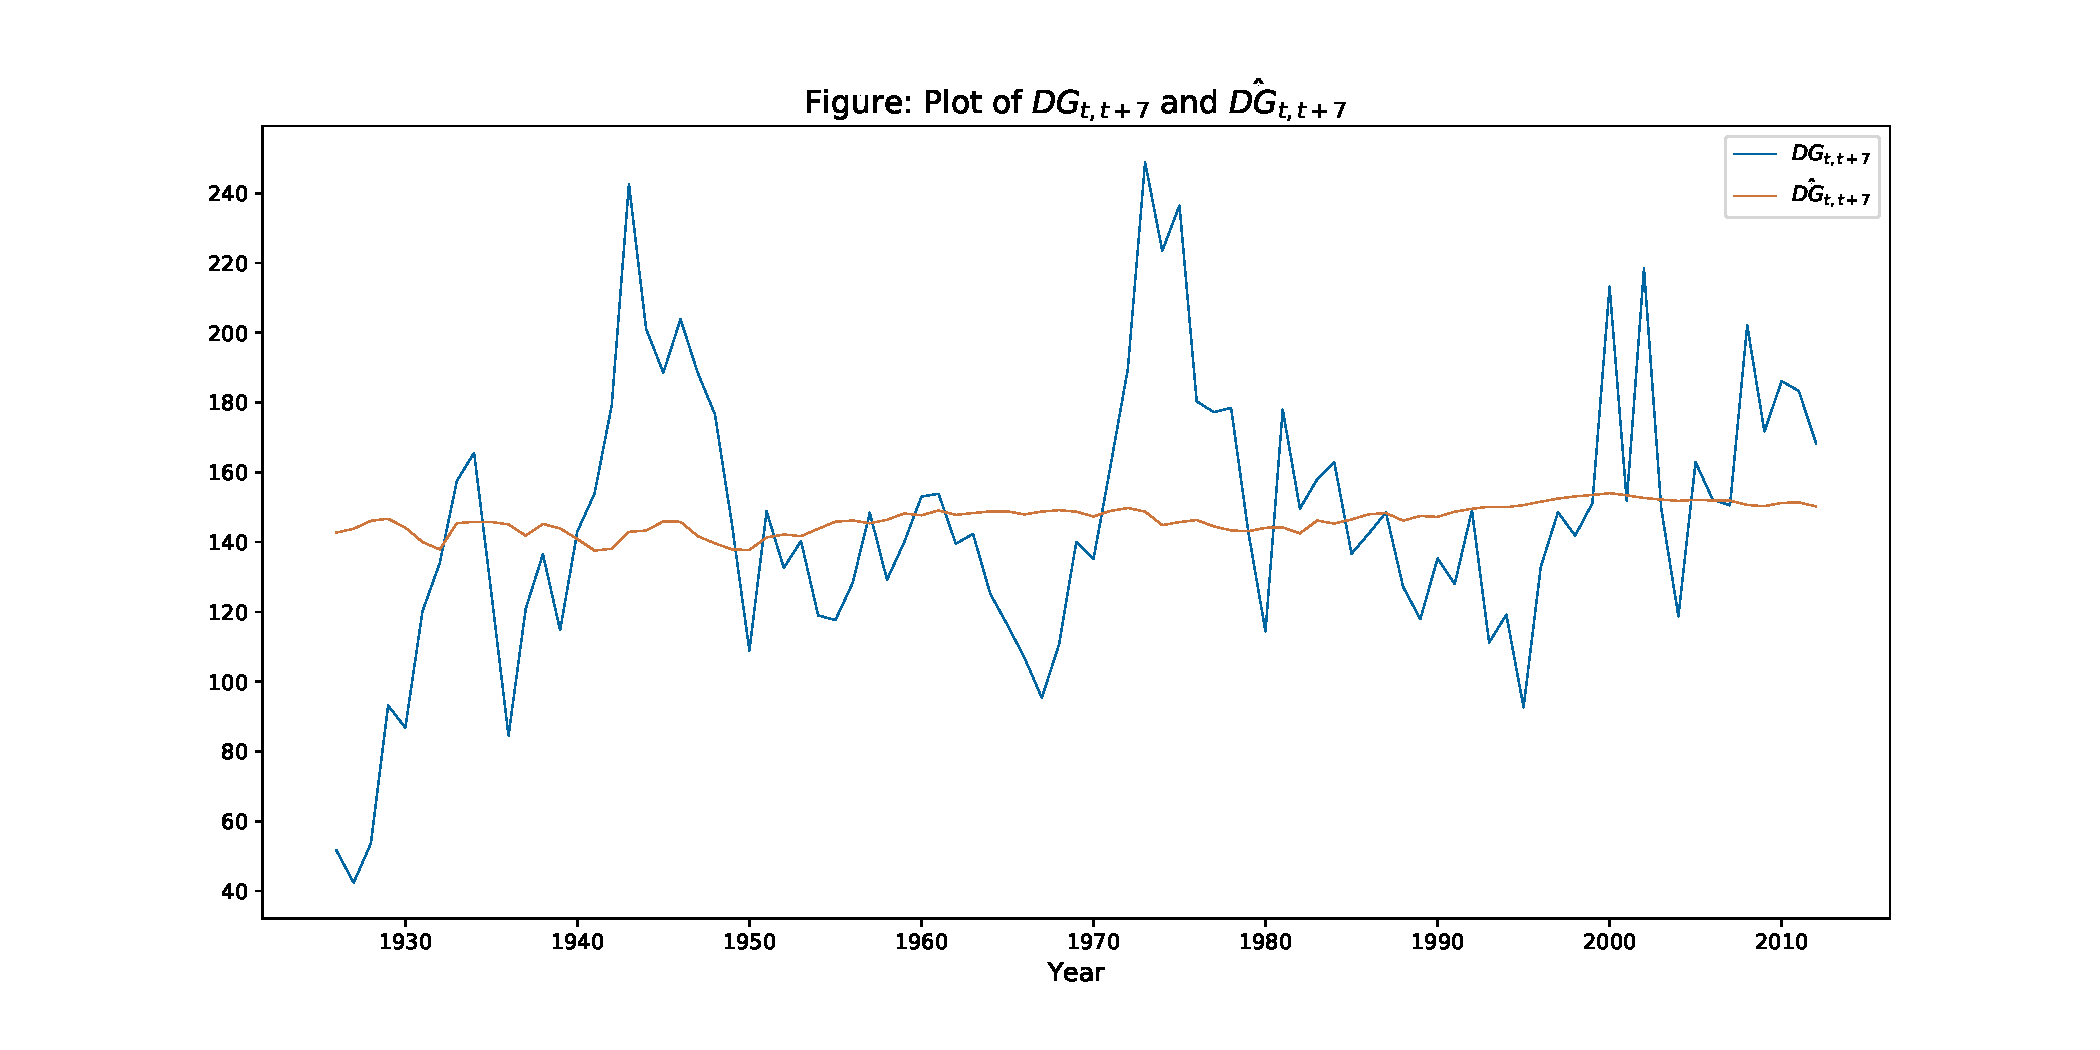
\includegraphics[width=\linewidth]{q2fig2.pdf}
\caption{This figure shows realized and predicted dividend growth. It suggests that dividend growth is not predictable.}
\end{figure}
\end{frame}




\begin{frame}{Q3: Multivariate forecast}
\begin{table}
\footnotesize
\begin{tabular}{lcccccccccc}
\toprule
& 1 & 2 & 3 & 4 & 5 & 6 & 7 & 8 & 9 & 10\\
\cmidrule{1-11}
$DP$ & 3.27 & 5.9 &  6.98 & 8.27 & 12.5 & 18.62 & 24.51 & 30.83 & 39.77 & 48.37 \\
$t$ & 1.63 & 1.49 & 1.41 & 1.67 & 2.37 & 2.74 & 3.58 & 4.31 &5.84 & 6.41 \\
$R^2$ & 0.03 & 0.05 & 0.05 & 0.04 & 0.07 & 0.13 & 0.18 & 0.20 & 0.25 & 0.28 \\
\cmidrule{1-11}
$cay$ & 1.88 & 4.51&  7.07 & 9.1 & 10.54& 12.17 & 12.47 & 14.61 & 18.73 & 22.17 \\
$t$ & 1.6 & 2.15 & 2.73 & 2.63 & 2.55 & 2.23 & 1.7 & 1.73 & 2.17 &2.55 \\
$R^2$ & 0.03 & 0.09 & 0.17 & 0.18 & 0.15 & 0.15 & 0.12 & 0.11 & 0.14 & 0.16 \\
\cmidrule{1-11}
$DP$ & 3.19 & 5.83 & 7.11 & 8.63 & 13.26 & 19.88 & 26.04 & 32.92 & 42.33 & 52 \\
$t_{DP}$ & 1.58 & 1.52 & 1.43 & 1.54 & 2.05 & 2.5 & 3.24 & 3.74 &4.57 & 5.77 \\
$cay$ & 1.83 & 4.48 &  7.12 & 9.22 & 10.89 & 12.9 & 13.55 & 16.18 & 20.65 & 24.91 \\
$t_{cay}$ & 1.59 & 2.19 & 2.69 & 2.70 & 2.87 & 3.31 & 2.71 & 3.36 &4.83 & 5.43 \\
$R^2$ & 0.05 & 0.14 & 0.22 & 0.24 & 0.23 & 0.3 & 0.32 & 0.35 & 0.43 & 0.5 \\
\bottomrule
\end{tabular}
\end{table}
\end{frame}



\begin{frame}{Q3: Multivariate forecast (cont'd)}
\begin{itemize}
  \item Observations:
  \begin{itemize}
    \item In this shorter sample (bacause $cay$ starts from 1952), the regression result are quite similar.
    \item The coefficients and $R^2$ for $cay$ and $DP$ are increasing through horizon $1-3$. However, after horizon $3$, the coefficients and $R^2$ for $cay$ becomes stable which implies that $cay$ is not persistent.
    \item $cay$ and $DP$ seem to complement with each other instead of substitute for each other. This relationship exists in all horizons.
  \end{itemize}
\end{itemize}
\end{frame}


\begin{frame}{Q3: Multivariate forecast (cont'd)}
\begin{figure}[h!]
\centering
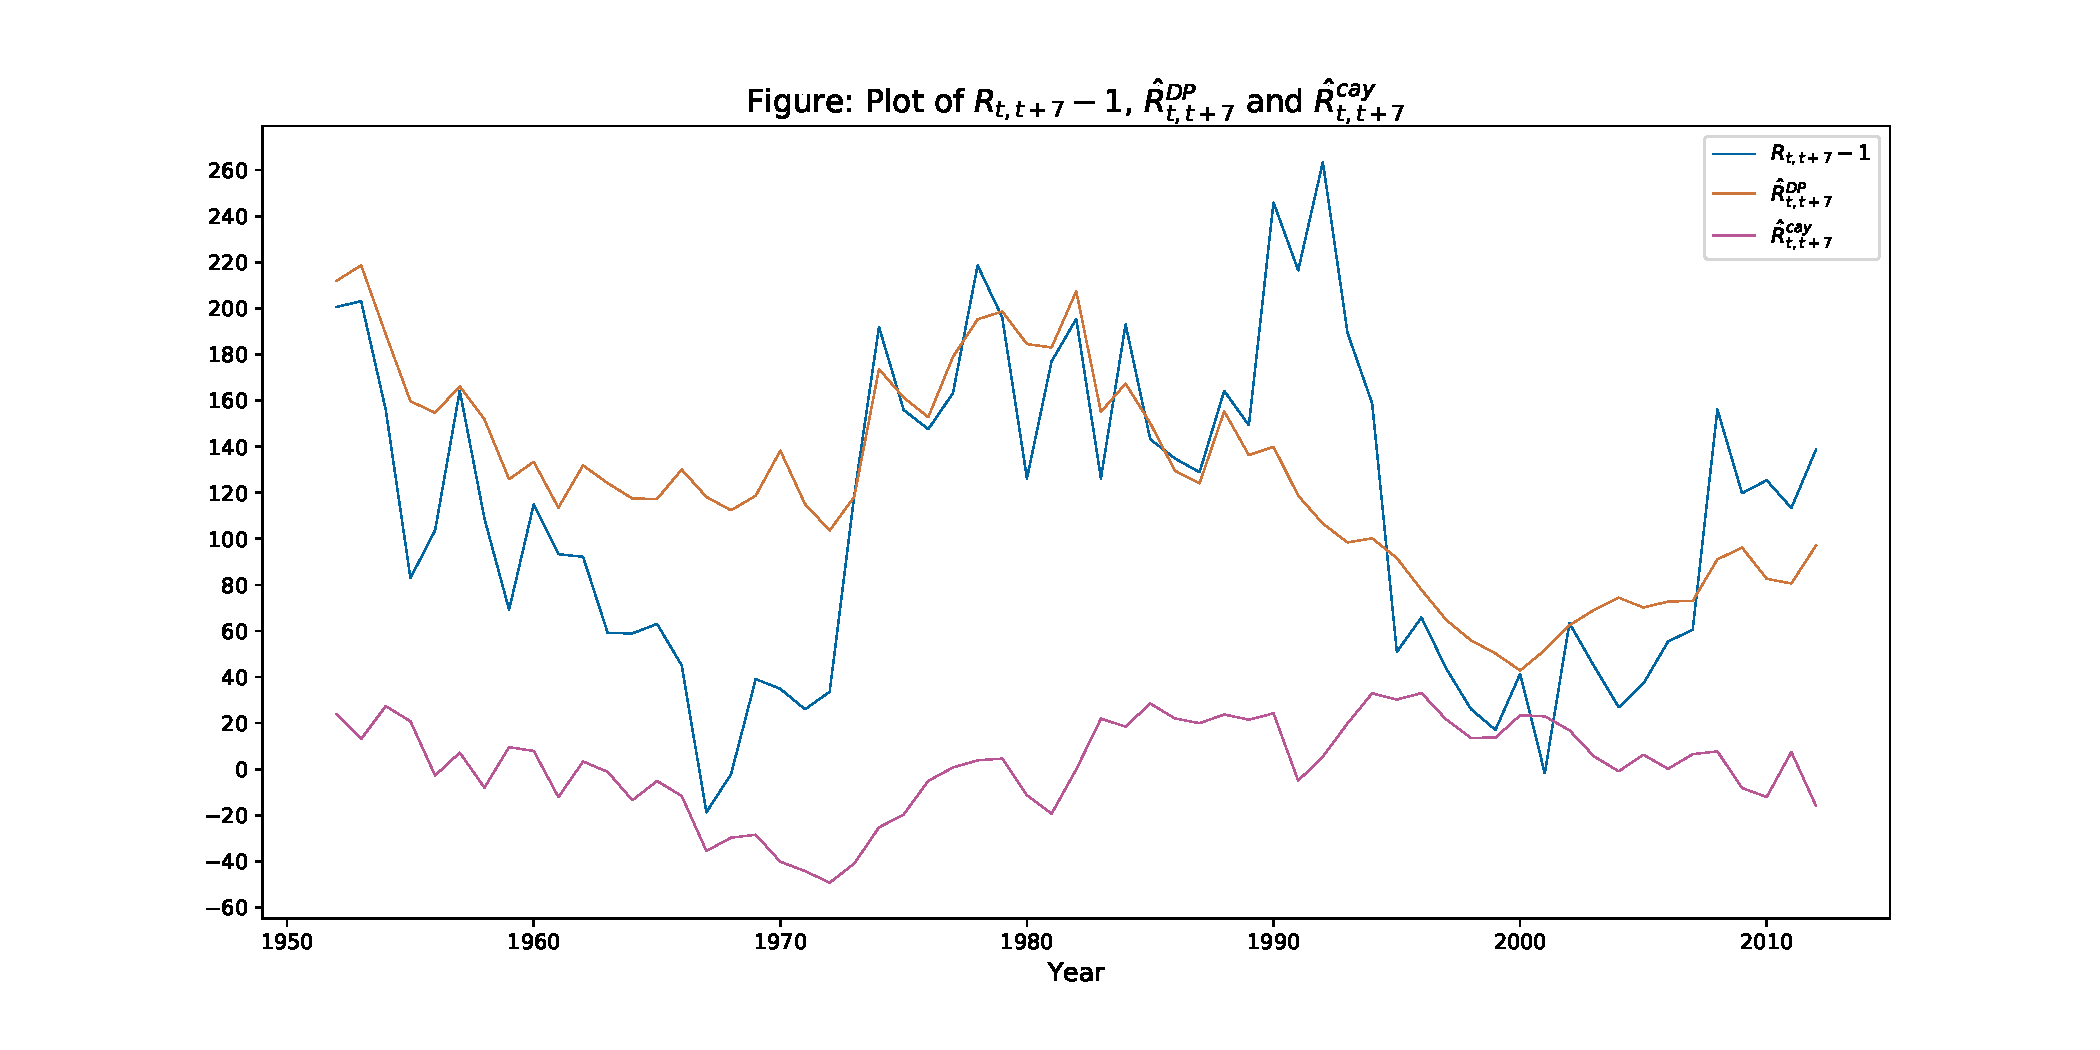
\includegraphics[width=\linewidth]{q3fig1.pdf}
\caption{$DP$ and $cay$ are complement in this way: $DP$ captures the slow-moving variation of returns, and $cay$ captures the quick-moving variations.}
\end{figure}
\end{frame}





\begin{frame}{Q4: Variance decomposition}
\begin{itemize}
  \item The log-linear approximation of $R_{t+1} = (P_{t+1} + D_{t+1})/P_{t}$ (omitting the constant term):
  $$
  \begin{array}[t]{rl}
  & r_{t+1} \approx \rho pd_{t+1} - pd_t + \Delta d_{t+1} \\
  \Leftrightarrow & \Delta d_{t+1} \approx r_{t+1} + \rho dp_{t+1} - dp_t, \text{ where } \rho = \exp(\bar{pd}) / (1 + \exp(\bar{pd}))
  \end{array}
  $$
  \item Using sample average ($\hat{\rho} = 0.97$), this identity becomes to be
  $$
  \Delta \hat{d}_{t+1} \approx r_{t+1} + 0.97 dp_{t+1} - dp_t
  $$
\end{itemize}
\end{frame}


\begin{frame}{Q4: Variance decomposition}
\begin{figure}[h!]
\centering
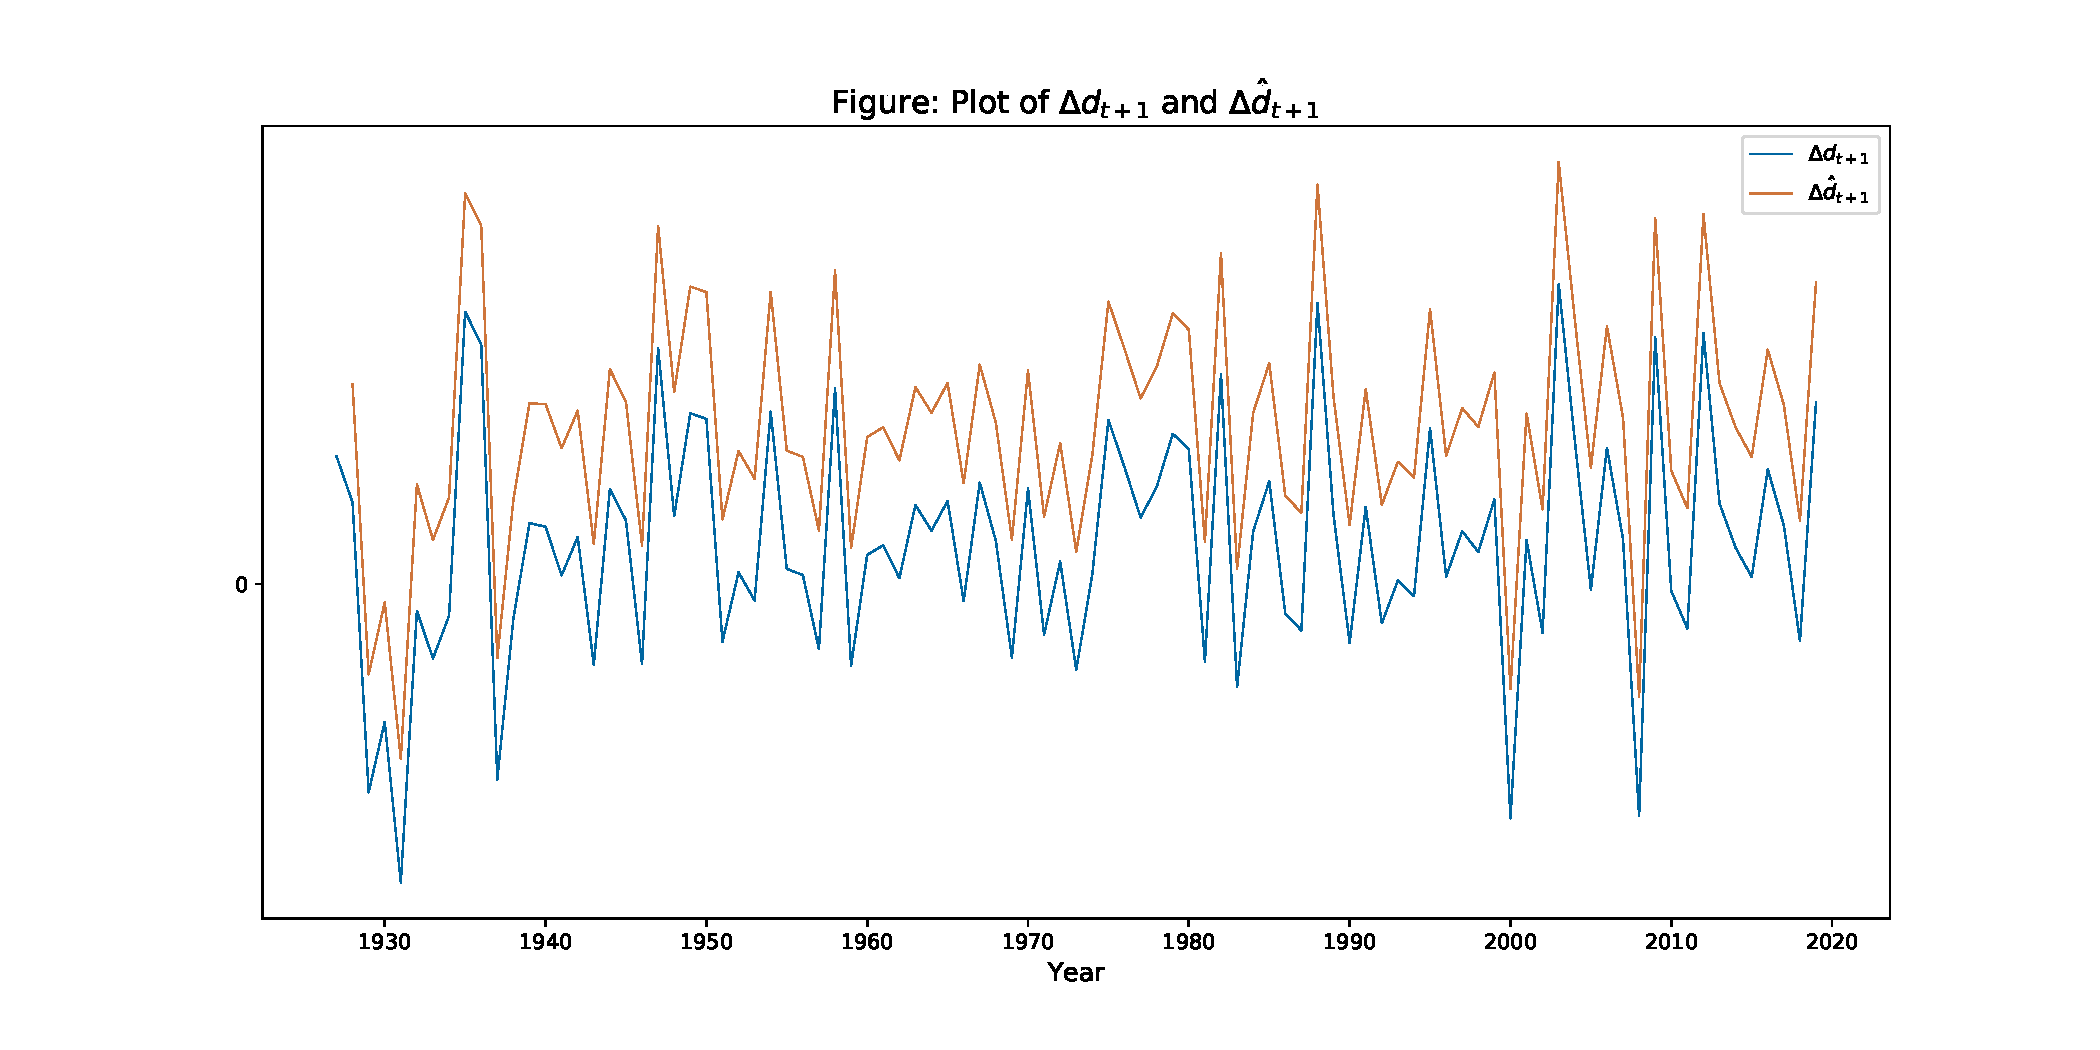
\includegraphics[width=\linewidth]{q4fig1.pdf}
\caption{This figure shows the dividend growth rate in data and dividend growth rate implied by log-return identity are the same.}
\end{figure}
\end{frame}




\begin{frame}{Q4: Variance decomposition (Cont'd)}
\begin{itemize}
  \item Suppose the state variables at $t$ are $X_t = (r_t, dp_t)^T$ which proceed following $VAR(1)$.
\begin{table}
\begin{tabular}{lccc}
\toprule
& $r_t$ & $dp_t$ & $\bar{R}^2$ \\
\cmidrule{1-4}
$r_{t+1}$ & 0.05 & 0.08 & 0.01 \\
$dp_{t+1}$ & -0.21 & 0.94 & 0.89 \\
\bottomrule
\end{tabular}
\end{table}
  \item $R^2$ for the return is low. But it is not a problem. Because from the plot, we can see that the realized return is quite volatile. It's plausible that the variation of expected return compared to the variation of the realized returns are low.
  \item $\sigma(E_{t}(r_{t+1}))$: $0.04$, $E(r_t)$: $0.09$. The magnitude of the variation in expected returns is nearly one-half of the unconditional expected returns and is economically significant.
\end{itemize}
\end{frame}


\begin{frame}{Q4: Variance decomposition (Cont'd)}
\begin{table}
\begin{tabular}{lccc}
\toprule
& $r_t$ & $dp_t$ & $\frac{\sigma^2()}{\sigma^2(dp_t)}$ \\
\cmidrule{1-4}
$e_1G$ & -0.12 & 0.8 & 0.65 \\
$e_dG$ & -0.12 & -0.2 & 0.04 \\
\bottomrule
\end{tabular}
\end{table}
\begin{itemize}
  \item Observations:
  \begin{itemize}
    \item $\frac{\sigma^2(pd^r_{t})}{\sigma^2(pd_t)} = 0.65$ and $\frac{\sigma^2(pd^d_{t})}{\sigma^2(pd_t)} = 0.04$ imply that most of variation in $dp$ associates the variation of long-run expected return instead of the long-run dividend growth.
    \item Long-run expected return is predictable.
  \end{itemize}
\end{itemize}
\end{frame}

\begin{frame}{Q4: Variance decomposition (Cont'd)}
\begin{itemize}
  \item $Cov(dp_t^r, dp_t^d) / Var(dp_t) = -0.16$. Long-run expected returns and dividend growth are negatively correlated. This implies that when investors anticipate a high dividend growth in the future, they require a less expected return.
  \item $Var(dp_t^r) + Var(dp_t^d) - 2Cov(dp_t^r, dp_t^d) = Var(dp_t)$.
  \item $X_t \subset \mathcal{F}_t$ does not matter. Because adding more variable as regressors will increase the regression's $R^2$, and thus reinforce the return predictability.
\end{itemize}
\end{frame}



\begin{frame}{Q5: Ito's lemma}
\begin{itemize}
  \item Diffusion model of $y_t$:
  $$
  \diff y_t = \mu \diff t + \sigma \diff w_t
  $$
  \item Using Ito's lemma, we can derive the diffusion model of $x_t = \exp(y_t)$:
  \begin{equation*}
  \begin{split}
  \diff x_t & = \big(\exp(y_t) \mu + \frac{1}{2} \exp(y_t) \sigma^2 \big) \diff t + \exp(y_t) \sigma \diff w_t \\
  & = \big(x_t \mu + \frac{1}{2} x_t \sigma^2 \big) \diff t + x_t \sigma \diff w_t \\
  & = \big(\mu + \frac{1}{2}\sigma^2 \big) x_t \diff t + \sigma x_t  \diff w_t
  \end{split}
  \end{equation*}
\end{itemize}
\end{frame}

\begin{frame}{Q5: Brownian motion}
\begin{itemize}
  \item From discrete-time to continuous-time stochatic processes:
  \begin{equation*}
  \begin{split}
  & w_{t+k} - w_t = \Sigma_{i = 1}^k \varepsilon_{t+i} \sim N(0, k) \\
  \Rightarrow & w_{t+\Delta t} - w_t \sim N(0, \Delta t) \\
  \Rightarrow & \diff w_t / \diff t \rightarrow +\infty
  \end{split}
  \end{equation*}
  \item Hence,
  \begin{equation*}
  \begin{split}
  &   \frac{(w_{t+\Delta t} - w_t)^2}{\Delta t} \sim \chi_1^2 \\
  \Rightarrow & E_t(w_{t+\Delta t} - w_t)^2 = \Delta t \\
  & Var_t(w_{t+\Delta t} - w_t)^2 = 2 \Delta^2 t \\
  \Rightarrow & (\diff w_t)^2 / \diff t \sim \chi_1^2
  \end{split}
  \end{equation*}
  \item The standard deviation is in the $\mathcal{O}(\Delta t)$ order, which will vanish as $\Delta t \rightarrow 0$.
\end{itemize}
\end{frame}

\begin{frame}{Q5: Brownian motion (cont'd)}
\begin{figure}[h!]
\centering
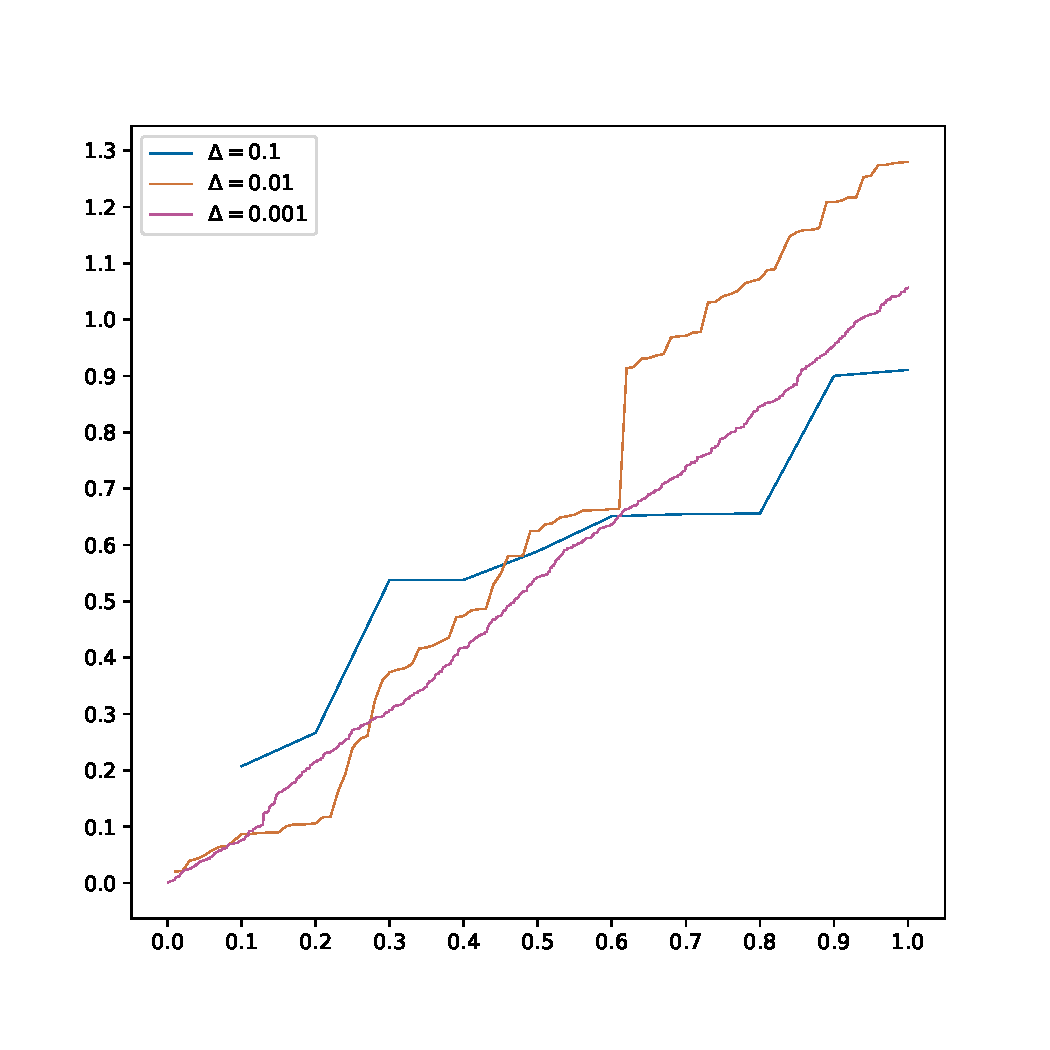
\includegraphics[width=0.5\linewidth]{q5fig1.pdf}
\caption{This figure shows that as $\Delta t$ becomes smaller, the cumulative sum of $(z_{t+\Delta} - z_t)^2$ converges to the straight line.}
\end{figure}
\end{frame}

\end{document}

